\section{Ex2.06 Plotting $1/x^n$}\label{1/x^n}
\subsection{Testo esercizio}
La funzione $f(x;n)$ è data come $f(x;n) =\frac{1}{x^{n}}$

\begin{itemize}
    \item[a)] Creare una funzione $fvalue(x,n)$ che restituisce il valore di $f(x,n)$.
        
    \item[b)] Usa questa funzione per tracciare $$f_1=\dfrac{1}{x},\quad 
    f_2=\dfrac{1}{x^2}, \quad f_3=\dfrac{1}{x^3}$$ nello stesso grafico per $-1<x<1$.
\end{itemize}

\subsection{Svolgimento}
L'esercizio è stato di base semplice. E' Bastato attenzionare \verb*|./| e \verb*|.^| per 
operare singolarmente su ogni elemento di matrici come se fosse un elemento a se stante e 
il resto è stato semplice.

\subsection{Risultato}
\begin{figure}[h]
    \centering
    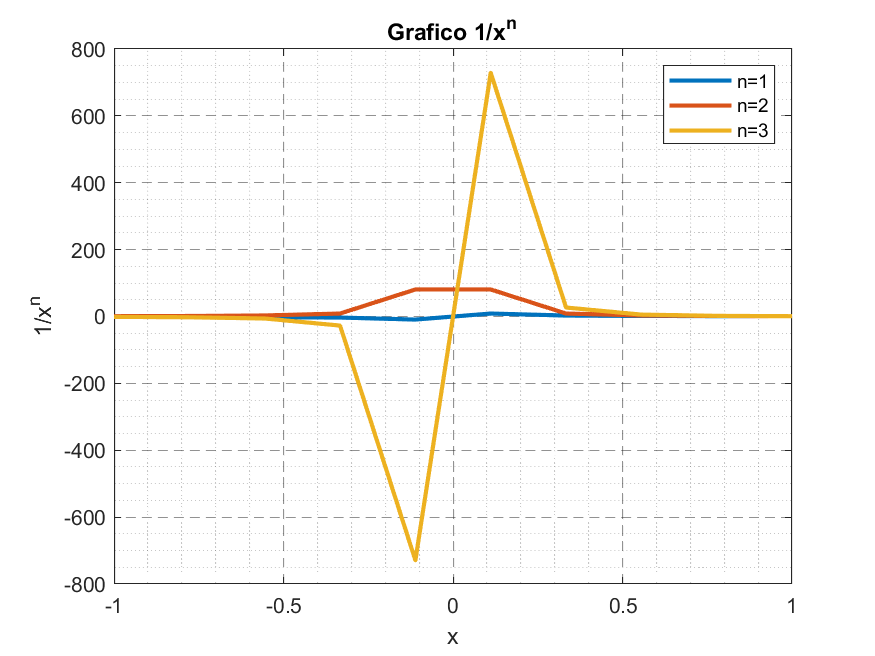
\includegraphics{cap/Elementary/img/script206}
    \GraphCap{$1/x^n$}
    \label{fig:script206}
\end{figure}
\newpage

\subsection{Codice esercizio}
\lstinputlisting[caption = {\nameref{fnc:fvalue}},
linerange={42-50}]
{cap/Elementary/src/function/fvalue.m}

\lstinputlisting[title = {Script Ex2.06}]
{cap/Elementary/src/script/script206.m}
